%t%%%%%%%%%%%%%%%%%%%%%%%%%%%%%%%%%%%%%%%%%
% NIWeek 2014 Poster by T. Reveyrand
% www.microwave.fr
% http://www.microwave.fr/LaTeX.html
% ---------------------------------------
% 
% Original template created by:
% Brian Amberg (baposter@brian-amberg.de)
%
% This template has been downloaded from:
% http://www.LaTeXTemplates.com
%
% License:
% CC BY-NC-SA 3.0 (http://creativecommons.org/licenses/by-nc-sa/3.0/)
%
%%%%%%%%%%%%%%%%%%%%%%%%%%%%%%%%%%%%%%%%%

%----------------------------------------------------------------------------------------
%	PACKAGES AND OTHER DOCUMENT CONFIGURATIONS
%----------------------------------------------------------------------------------------

\documentclass[a0paper,portrait]{baposter}

%%%% Font stuff begins
\usepackage[T1]{fontenc}
\usepackage{frutiger}	 		  % Fraunhofer official font
\usepackage{microtype}
\DisableLigatures[f]{encoding=T1} % Disable ligatures because font doesn't have it
%%%% Font stuff ends

\usepackage[font=small,labelfont=bf]{caption} % Captions for tables and figures
\usepackage{multirow} % Multiple rows in tables
\usepackage{array}    % Better table alignment
\usepackage{booktabs} % Horizontal rules in tables
\usepackage{enumitem} % Improved enumerate and listings
\usepackage{relsize}  % Used for making text smaller in some places
\usepackage{amsmath,amsfonts,amssymb,amsthm} % Math packages
\usepackage{siunitx}  % Units
\usepackage{eqparbox}
\usepackage{textcomp}
\usepackage{xcolor, colortbl}
\usepackage{graphicx}
\usepackage{pdfpages}
\usepackage[retainorgcmds]{IEEEtrantools}
\usepackage{pgfplots}
\pgfplotsset{compat=newest}
\usepgfplotslibrary{fillbetween}
\usepackage{csquotes} % Quotation marks

%% the following commands are needed for some matlab2tikz features
\usetikzlibrary{plotmarks}
\usetikzlibrary{arrows.meta}
\usepgfplotslibrary{patchplots}
\usepackage{grffile}
% Tikz
\usepackage{tikz}
\usepackage{circuitikz}[european]
\usetikzlibrary{shapes}
\usetikzlibrary{calc, intersections, arrows, shapes}

\graphicspath{{figures/}} % Directory in which figures are stored
\setlist[itemize]{noitemsep, topsep=0pt}  % remove spacing in enumerates

%\definecolor{fhggreen}{RGB}{23,156,125}
\definecolor{fhggreen}{RGB}{23,200,90}
\definecolor{fhggrey}{RGB}{225,227,227}
\definecolor{fhgdarkgrey}{RGB}{168,175,175}
\definecolor{fhglightgrey}{RGB}{235,238,238}
\definecolor{IRPblue}{rgb}{0.4588,0.4196,0.6941}%
\definecolor{MPCgreen}{rgb}{0.1922,0.6392,0.3294}%
\definecolor{headerfontcol}{RGB}{0,0,0} % Header text color - black
 
\usepackage{lmodern} 
\newlength\figureheight
\newlength\figurewidth 
\setitemize{leftmargin=*}

\renewcommand{\familydefault}{\sfdefault}
\usepackage[cm]{sfmath}			  % Sans Serif math fonts, must come after \sfdefault


\begin{document}

%%%%%%% MORE FONT STUFF
\usefont{T1}{pfr}{l}{n}\selectfont							%Use Frutiger font
%%%%%%% END?

\renewcommand{\labelitemi}{\scriptsize$\blacksquare$}		%Square for itemize env.
%\def\matlab{MATLAB }
\def\simulink{SIMULINK }
\newcommand{\bbma} {\begin{bmatrix} }
\newcommand{\ebma} {\end{bmatrix}}
\newcommand{\bpma} {\begin{pmatrix} }
\newcommand{\epma} {\end{pmatrix}}


 \def\vec#1{\ensuremath{\mathchoice
                     {\mbox{\boldmath$\displaystyle\mathbf{#1}$}}
                     {\mbox{\boldmath$\textstyle\mathbf{#1}$}}
                     {\mbox{\boldmath$\scriptstyle\mathbf{#1}$}}
                     {\mbox{\boldmath$\scriptscriptstyle\mathbf{#1}$}}}}%

% tensor
\def\tens#1{\relax\ifmmode\mathsf{#1}\else\textsf{#1}\fi}

\def\norm#1{\|#1\|} 

\def\utilde{\undertilde}

%\def\kruskal#1{\left[\left[\; #1 \;\right]\right]}

\newcommand{\tucker}[2]{\left[ #1 \right] \cdot #2}
\newcommand{\kruskalone}[1]{\left[ #1 \right] \cdot \tens{I}}
\newcommand{\kruskal}[2]{\left[ #1 \right] \cdot #2 }
\newcommand{\krusk}[1]{\left[ #1 \right] }
\newcommand{\kruskaltwo}[2]{\left[ #1 \right] \cdot #2}

%\newcommand{\cprod}[3]{\left\langle\!\!\!\left\langle \, #1 \,|\,  #2  \right.\right\rangle_{#3}}

%\newcommand{\cprod}[3]{\left\langle #1 \,,\,  #2  \right\rangle_{#3}}

\newcommand{\cprod}[3]{\left\langle\,#1\,\left|\,#2\,\right.\right\rangle_{#3}}
\newcommand{\aprod}[3]{\left\langle\,#1\,\left|\,#2\,\right.\right\rangle^+_{#3}}
\newcommand{\bprod}[3]{\left\langle\,#1\,\left|\,#2\,\right.\right\rangle^\Box_{#3}}
\newcommand{\hprod}[3]{\left\langle\,#1\,\left|\,#2\,\right.\right\rangle^\boxplus_{#3}}

%\newcommand{\cprod}[3]{\left\langle\,#1\,|\cdot |\,#2\,\right\rangle_{#3}}


%\newcommand{\hprod}[3]{\left\langle\!\left\langle #1 \,|\, #2  \right.\right\rangle^*_{#3}}

\newcommand{\iprod}[2]{\left\langle #1 \,,\,  #2  \right\rangle}

\newcommand{\btens}[1]{ 
\underline{\tens{#1}}}

\newcommand{\htens}[1]{ 
{\tens{#1}^*}}

\newcommand{\ctens}[1]{ 
\utilde{\tens{#1}}}

%\newcommand{\atens}[1]{ 
%\underline{\underline{\tens{#1}}}}

\newcommand{\atens}[1]{ 
\tens{#1}}

\newcommand{\cvec}[1]{%\raisebox{1mm}{
\utilde}
}}

%commands for scalars 
\newcommand{\cscal}[1]{%\raisebox{1mm}{
\utilde}
}}
\newcommand{\bscal}[1]{%\raisebox{1mm}{
\underline}
}}

\newcommand{\amat}[1]{ 
\underline{\underline{\mat{#1}}}}

%\newcommand{\amati}[1]{ 
%\underline{\underline{\mat{#1}\hspace{-1pt}}}\hspace{1pt}}

\newcommand{\amati}[1]{ 
\mat{#1}}


\newcommand{\cmat}[1]{%\raisebox{1mm}{
\utilde}
}}


\newcommand{\btensi}[1]{ 
\underline{\tens{#1}\hspace{-1pt}}\hspace{1pt}}


\newcommand{\ctensi}[1]{ 
\utilde{\tens{#1}\hspace{-1pt}}\hspace{1pt}}

\newcommand{\bvec}[1]{ 
\underline{\vec{#1}}}



\newcommand{\bveci}[1]{
\underline{\vec{#1}\hspace{-1pt}}\hspace{1pt}}



\newcommand{\tmat}[1]{\mbox{mat} \left( 
\mathbf{#1} \right)}

\newcommand{\tvec}[1]{\mbox{vec} \left( 
\mathbf{#1} \right)}

\newcommand{\hvec}[1]{ \mathbf{#1}}


%\newcommand{\fone}[0]{\vec{\nu}_1 }
%\newcommand{\fzero}[0]{\vec{\nu}_0 }
%\newcommand{\fdcare}[0]{\vec{\nu}_{-}}

%\newcommand{\fone}[0]{\boxminus_1 }

\newcommand{\fone}[0]{\framebox[4mm]{1}}
\newcommand{\fzero}[0]{\framebox[4mm]{0}}
%\newcommand{\fdcare}[0]{\framebox[4mm]{\phantom{$0$}\hspace{-5pt}$-$}}
\newcommand{\fdcare}[0]{\framebox[4mm]{\phantom{$0$}}}



\newcommand{\mat}[1]{
\mathbf{#1}}

\newcommand{\bmati}[1]{ 
\underline{\mathbf{#1}\hspace{-1pt}}\hspace{1pt}}

\newcommand{\bmat}[1]{ 
\underline{\mathbf{#1}}}


\newcommand{\bighadamard}
{ \bigotimes\hspace{-3.26ex}\bigoplus}

\newcommand{\hadamard}
{\circledast}
%{ \otimes\hspace{-2.03ex}\oplus\;}

\newcommand{\vecop}[1]
{ \mbox{vec}\hspace{1mm}({#1}) }

\newcommand{\mycitation}[2]
{
\vspace{-25mm}
\hfill
\begin{minipage}[t]{0.45\textwidth}
\textit{#1}
\end{minipage}
\vspace{5mm}

\hfill \textrm{#2}

\vspace{15mm}
}


\newcommand{\tikzfig}[4]
{
\begin{figure}[h!]
\begin{center}
\scalebox{#3}{
\input{../pic/#2/#1.tikz}
%Figure
}
\end{center}
\caption{#4}
\label{fig:#2--#1}
\end{figure}
}


\newcommand{\myfig}[4]
{
\begin{figure}[h!]
\begin{center}
\ifpdf
	\includegraphics[scale = #3]{../pic/#2/#1.pdf}
\else
	\includegraphics[scale = #3]{../pic/#2/#1.eps}
\fi
%Figure
\end{center}
\caption{#4}
\label{fig:#2--#1}
\end{figure}
}

%%%%%MTI functions
\newcommand{\monT}[1]{\tens{M}\left(#1\right)}
\newcommand{\monTN}[2]{\tens{M}_p^{#1}\left(#2\right)}
\newcommand{\monElTN}[2]{m_p^{#1}\left(#2\right)}
\newcommand{\LieSingle}[3]{\tens{L}_{#1,#2,#3}}
\newcommand{\LieDouble}[4]{\tens{L}_{#1,#2,#3,#4}}
\def\DiffMat{\mat{\Theta}}
\def\DiffMatEl{\Theta}


%%% Definition f�r die Iterationen beim ILC
\newcommand{\xd}[1]{#1_{d}}
\newcommand{\xdi}[1]{#1_{d+1}}
\newcommand{\xdnext}[1]{#1_{d,next}}
\newcommand{\xdii}[1]{#1_{d+2}}
\newcommand{\xdb}[1]{#1_{d,db}}
\newcommand{\xdbi}[1]{#1_{d+1,db}}
\newcommand{\xdbii}[1]{#1_{d+2,db}}


\background{ % Set the background to an image (background.pdf)
%\begin{tikzpicture}[remember picture,overlay]
%\draw (current page.north west)+(-2em,2em) node[anchor=north west]
%{\includegraphics[height=1.1\textheight]{background}};
%\end{tikzpicture}
}

\begin{poster}{
grid=false,				 % Grid for debugging/Layout testing
columns=3,				 % Change this for different column design
eyecatcher=true,		 % Logo on the left
headerheight=0.19\textheight,
boxpadding=1em,
borderColor=fhggreen,    % Border color of content boxes
headerColorOne=fhggrey,  % Background color header in the content boxes (left side)
headerColorTwo=fhggrey,  % Background color header in the content boxes (right side)
headerFontColor=headerfontcol, % Text color for the header text in the content boxes
boxColorOne=fhggrey,     % Background color for the content in the content boxes
textborder=rectangle,
headershape=rectangle,   % Specify the rounded corner in the content box headers
headerfont=\Large\sf\bf, % Font modifiers for the text in the content box headers
textborder=rectangle,
background=none,
headerborder=open, 		 % Change to closed for a line under the content box headers
boxshade=plain,
headershade=plain
}
{% Fraunhofer Logo
\makebox[0pt][t]{%
	\raisebox{3.7em}[0pt][0pt]{%
		
\includegraphics[width=5cm]{HAW_logo}}}
}
%
%----------------------------------------------------------------------------------------
%	TITLE AND AUTHOR NAME
%----------------------------------------------------------------------------------------
%
{\vspace*{2.1em} \\ \huge{Power Quality Compensation for Smart Grids by Model-based Predictive Control }} % Poster title
{\vspace{.4em} \smaller\textbf{Carlos Cateriano Y\'a\~nez\textsuperscript{1,2}, Kathrin Weihe\textsuperscript{1}, Georg Pangalos\textsuperscript{2}, and Gerwald Lichtenberg\textsuperscript{1}}  \\  % Author names
  
\vspace{.4em}\normalsize{\textsuperscript{1}Hamburg University of Applied Sciences, Faculty Life Sciences, Ulmenliet 20, 21033 Hamburg \\
\textsuperscript{2}Fraunhofer ISIT, Application Center Power Electronics for Renewable Energy Systems, Steindamm 94, 20099 Hamburg} \\ \normalsize{\vspace{.3em}{\{carlos.caterianoyanez, kathrinjoungah.weihe, gerwald.lichtenberg\}@haw-hamburg.de, georg.pangalos@isit.fraunhofer.de, }}  } % Author email addresses
{% Conference Logo
\makebox[0pt][t]{%
	\raisebox{4em}[0pt][0pt]{%
	\hspace*{-15.5cm}
	{\begin{tabular}{m{9.6cm} m{7cm}}
		\vspace{-1cm} 
\includegraphics[width=7.5cm]{dies_academicus}&
		\vspace{-1cm} 
\includegraphics[width=5.5cm]{_logo}
	\end{tabular}}}}
}

%----------------------------------------------------------------------------------------
%	Introduction
%----------------------------------------------------------------------------------------
\headerbox{INTRODUCTION}{name=intro,column=0,row=0, span=3}{
\vspace{-2em}
\textbf{
\begin{itemize}[itemsep=0pt]
\item High order harmonics in the electrical grid introduced by switching converters need to be compensated to avoid damage and energy loss
\item Classic active power filter (APF) controllers are capable of compensating harmonics, but are not flexible under variable load scenarios
\item A classic well-tested method to compensate harmonics relies on the instantaneous reference frame (IRP) theory
\item A novel approach: \enquote{Linear State Signal Shaping Model Predictive Control} (LSSS MPC), could be utilized to compensate harmonics using shape classes, without the need to design filters for different load scenarios
\end{itemize}
\vspace{-1.3em}
}}

%----------------------------------------------------------------------------------------
%	Application problem
%----------------------------------------------------------------------------------------
\headerbox{APPLICATION PROBLEM}{name=irpmpc,column=0,row=1,below=intro,span=2}{
\vspace{-2em}
\textbf{
\begin{itemize}[itemsep=0pt]
\item Could the LSSS MPC controller improve the grid quality compared to a standard IRP APF controller?
\item A simulation is set up to evaluate both controller types under different load scenarios
\end{itemize}}
\vspace{-1.2em}
}

%----------------------------------------------------------------------------------------
%	Classical Controller
%----------------------------------------------------------------------------------------
\headerbox{CLASSIC IRP CONTROLLER}{name=irp_block,column=0,row=1,below=irpmpc,span=1}{
%\vspace{.2em}
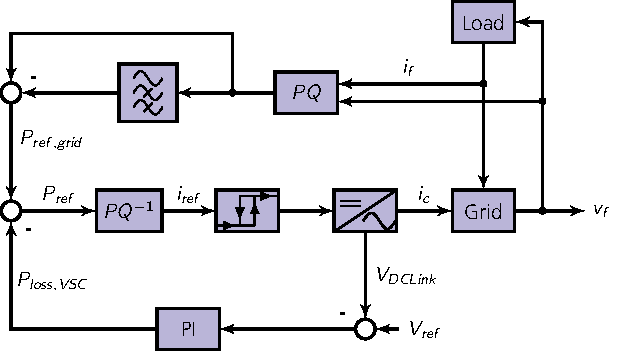
\includegraphics[scale=0.68]{irp_block}
\vspace{-.67em}
\textbf{
\begin{itemize}[itemsep=0pt]
\item Clarke and p-q transformation are used
\item A high pass filter extracts harmonics
\item A hysteresis band controller steers the voltage source converter
\end{itemize}}
}

%----------------------------------------------------------------------------------------
%	Predictive Controller
%----------------------------------------------------------------------------------------
\headerbox{PREDICTIVE CONTROLLER}{name=mpc_block,column=1,row=1,below=irpmpc,span=1}{
\vspace{-.4em}
\textbf{An MPC solves the optimization problem}
\vspace{-.3em}
\begin{equation*}
\min_{\Delta U} \Vert\mathbf{X}(k)-\Xi(k)\Vert^2_{\mathbf{Q}}+\Vert\Delta\mathbf{U}(k)\Vert^2_{\mathbf{R}}.
\end{equation*}
\vspace{-1.8em}
\begin{flushleft}
\textbf{An internal model enables prediction. The~unconstrained solution leads to a linear closed loop behaviour.}
\end{flushleft}
\vspace{-.4em}
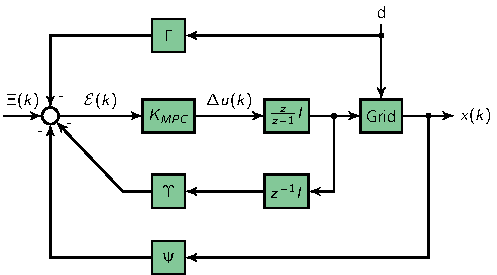
\includegraphics[scale=0.85]{mpc_block}
\vspace{-1.55em}
}

%----------------------------------------------------------------------------------------
%	Linear Shape Class
%----------------------------------------------------------------------------------------
\headerbox{LINEAR SHAPE CLASS}{name=mpc_block,column=1,row=2,below=mpc_block,span=1}{
\vspace{-.7em}
\textbf{The shape of a sine wave is described by the homogeneous ODE}
\vspace{-.3em}
\begin{equation*}
\frac{\text{d}^2x(t)^2}{\text{d}t} + \omega^2 x(t) = 0
\end{equation*}
\vspace{-.1em}
\textbf{and approximated in discrete time with}

\vspace{.7em}
\mbox{\large
$\frac{\left( 2 + \omega^2 t^{2}_{s} \right)x(k)-5x(k+1)+4x(k+2)-x(k+3)}{t^{2}_{s}} = 0.$}

\vspace{.5em}
\textbf{From this difference equation the \textit{linear shape class\textsuperscript{3}}{\renewcommand*\@makefnmark{}\footnote{\textsuperscript{3}Cateriano Y\'a\~nez, C., Pangalos, G., and Lichtenberg, G. (2018). An approach to linear state signal shaping by quadratic model predictive control. In \textit{European Control Conference (ECC) 2018 \vspace{-.4em}}}\makeatother} $\mathbf{V}$ is given as}
%\vspace{-.5em}
\begin{equation*}
\mathbf{V} = 
\left( \begin{array}{cccc} 
2+(\omega t_s)^2 & 5 & 4 & - 1
\end{array} \right)\in \mathbb{R}^{1 \times 4} \; .
\end{equation*}

\textbf{The state error weight matrix $\mathbf{Q}$ is built using $\mathbf{V}$ by transferring the control goal to the optimization problem}
\vspace{-.2em}
\begin{equation*}
\min_{\mathbf{X}(k)} \left( \mathbf{V}\mathbf{X}(k) \right)^2,
\end{equation*}

\vspace{-.7em}
\textbf{where}
\small
\begin{equation*} 
\mathbf{X}(k) =  \left(\begin{array}{cccc} x(k) & x(k+1) & x(k+2) & x(k+3) \end{array} \right)^\intercal\!,
\end{equation*}
\normalsize
\textbf{for all times $k$.}

\vspace{.56em}
}


%----------------------------------------------------------------------------------------
%	Three-phase three-node grid model
%----------------------------------------------------------------------------------------

\headerbox{3-PHASE GRID MODEL}{name=gridmodel,column=0,row=2,below=irp_block,span=1}{

\vspace{-.17em}
\begin{center}
%\input{figures/gridmodel.tikz}
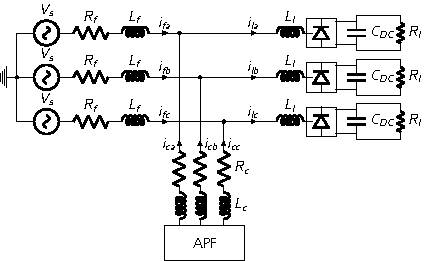
\includegraphics{gridmodel}
\end{center}

\textbf{Active power filter in shunt configuration}

}

%----------------------------------------------------------------------------------------
%	White-Box Modeling
%----------------------------------------------------------------------------------------
\headerbox{WHITE-BOX MODELING}{name=ssmodel,column=0,row=3,below=gridmodel,span=1}{
\vspace{-.2em}
\begin{flushleft}
\textbf{Linear state space model of the grid} \end{flushleft}
\vspace{-.7em}
\begin{IEEEeqnarray*}{rCl}
\mathbf{\dot{x}}(t)& = &\mathbf{A}\mathbf{x}(t)+\mathbf{B}\mathbf{u}(t)+\mathbf{E}\mathbf{d}(t)
\end{IEEEeqnarray*}
\vspace{-.7em}
\textbf{where}
\vspace{-.65em}
\begin{IEEEeqnarray*}{rCl}
\mathbf{x}(t)  &= & \begin{pmatrix}
v_l & \frac{di_c}{dt} & \frac{di_{l}}{dt} 
\end{pmatrix}^\intercal \in \mathbb{R}^3 \quad 
\arraycolsep=1.1pt\def\arraystretch{1.5}
\begin{array}{rcl}u(t)&=& \frac{\text{d}^2i_c}{\text{d}t^2}\\d(t)&=&\frac{\text{d}^2i_l}{\text{d}t^2} \end{array}
\end{IEEEeqnarray*}
\vspace{-.7em}
%\textbf{with the system matrix} $\mathbf{A} \in \mathbb{R}^{3\times 3}$\textbf{, the input matrix} $\mathbf{B} \in \mathbb{R}^{3\times 1}$ \textbf{and the state disturbance matrix} $\mathbf{E} \in \mathbb{R}^{3\times 1}$.
\textbf{and}
\begin{equation*}
\mathbf{A} \in \mathbb{R}^{3\times 3}, \quad \mathbf{B} \in \mathbb{R}^{3\times 1}, \quad \mathbf{E} \in \mathbb{R}^{3\times 1}.
\end{equation*}
\vspace{-2em}
}
%----------------------------------------------------------------------------------------
%	Simulation Studies
%----------------------------------------------------------------------------------------

\headerbox{SIMULATION STUDIES}{name=simresult,column=2,row=1,below=intro,span=1}{
\vspace{-.5em}
\textbf{IRP APF harmonic current compensation:}
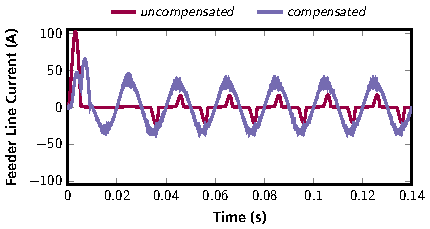
\includegraphics{pqif}

\textbf{LSSS MPC harmonic current compensation:}
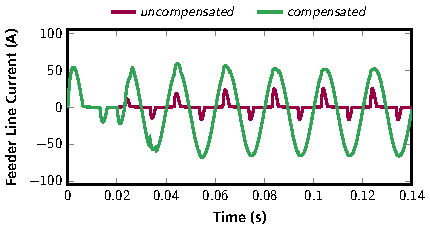
\includegraphics{mpcif}

\vspace{-.4em}
\begin{flushleft}
\textbf{Total harmonic distortion (THD):}
\end{flushleft}
\vspace{-.6em}
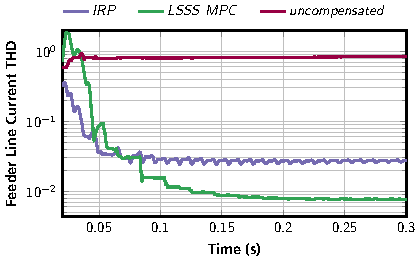
\includegraphics{thd} \\

\vspace{-1.7em}
\begin{flushleft}
\textbf{Results for different load scenarios:} \end{flushleft}

\vspace{.4em}
\newcolumntype{i}{>{\columncolor{IRPblue!50}}c}
\newcolumntype{j}{>{\columncolor{MPCgreen!50}}c}
\textbf{\footnotesize{
{\renewcommand{\arraystretch}{1.5}
\renewcommand{\tabcolsep}{0.2cm}
\setlength\arrayrulewidth{1.2pt}
\begin{tabular}{|c|i|j|i|j|}
\hline
\rowcolor{fhgdarkgrey}
\multirow{2}{*}{\begin{tabular}[c]{@{}c@{}}Load \\scenario \end{tabular}} & \multicolumn{2}{c|}{\textit{THD} ($v_f$)} & \multicolumn{2}{c|}{\textit{THD} ($i_f$)} \\ \cline{2-5} 
  & IRP          & MPC          & IRP          & MPC          \\ \hline
\cellcolor{fhgdarkgrey}\SI{100}{\ohm}           & 0.65\%       & 0.17\%       & 4.35\%       & 0.78\%       \\ \hline
\cellcolor{fhgdarkgrey}\SI{9}{\ohm}             & 0.45\%       & 0.35\%       & 0.75\%       & 1.57\%       \\ \hline
\cellcolor{fhgdarkgrey}\SI{2}{\ohm}             & 1.15\%       & 0.35\%       & 3.75\%       & 1.33\%       \\ \hline
\end{tabular}}}}
\vspace{-.35em}
}

%----------------------------------------------------------------------------------------
%	Conclusion
%----------------------------------------------------------------------------------------

\headerbox{CONCLUSION}{name=conclusion,column=2,row=2,below=simresult,span=1}{
\vspace{-1.6em}
\textbf{
\begin{itemize}[itemsep=0pt]
\item The LSSS MPC approach has the potential to successfully control an APF
\item Classic IRP controllers rely on high pass filter design to achieve good compensation results in a given load scenario
\item The LSSS MPC is capable of adapting to a wider variety of load scenarios
\end{itemize}}
\vspace{-1.0em}
}

\end{poster}

\end{document}